\documentclass[journal,12pt,twocolumn]{IEEEtran}
\usepackage{setspace}
\usepackage{gensymb}
\usepackage{xcolor}
\usepackage{caption}
\singlespacing
\usepackage{siunitx}
\usepackage[cmex10]{amsmath}
\usepackage{mathtools}
\usepackage{hyperref}
\usepackage{amsthm}
\usepackage{mathrsfs}
\usepackage{txfonts}
\usepackage{stfloats}
\usepackage{cite}
\usepackage{cases}
\usepackage{subfig}
\usepackage{longtable}
\usepackage{multirow}
\usepackage{enumitem}
\usepackage{bm}
\usepackage{mathtools}
\usepackage{listings}
\usepackage{tikz}
\usetikzlibrary{shapes,arrows,positioning}
\usepackage{circuitikz}
\renewcommand{\vec}[1]{\boldsymbol{\mathbf{#1}}}
\DeclareMathOperator*{\Res}{Res}
\renewcommand\thesection{\arabic{section}}
\renewcommand\thesubsection{\thesection.\arabic{subsection}}
\renewcommand\thesubsubsection{\thesubsection.\arabic{subsubsection}}

\renewcommand\thesectiondis{\arabic{section}}
\renewcommand\thesubsectiondis{\thesectiondis.\arabic{subsection}}
\renewcommand\thesubsubsectiondis{\thesubsectiondis.\arabic{subsubsection}}
\hyphenation{op-tical net-works semi-conduc-tor}

\lstset{
language=Python,
frame=single, 
breaklines=true,
columns=fullflexible
}
\begin{document}
\theoremstyle{definition}
\newtheorem{theorem}{Theorem}[section]
\newtheorem{problem}{Problem}
\newtheorem{proposition}{Proposition}[section]
\newtheorem{lemma}{Lemma}[section]
\newtheorem{corollary}[theorem]{Corollary}
\newtheorem{example}{Example}[section]
\newtheorem{definition}{Definition}[section]
\newcommand{\BEQA}{\begin{eqnarray}}
\newcommand{\EEQA}{\end{eqnarray}}
\newcommand{\define}{\stackrel{\triangle}{=}}
\newcommand{\myvec}[1]{\ensuremath{\begin{pmatrix}#1\end{pmatrix}}}
\newcommand{\mydet}[1]{\ensuremath{\begin{vmatrix}#1\end{vmatrix}}}
\bibliographystyle{IEEEtran}
\providecommand{\nCr}[2]{\,^{#1}C_{#2}} % nCr
\providecommand{\nPr}[2]{\,^{#1}P_{#2}} % nPr
\providecommand{\mbf}{\mathbf}
\providecommand{\pr}[1]{\ensuremath{\Pr\left(#1\right)}}
\providecommand{\qfunc}[1]{\ensuremath{Q\left(#1\right)}}
\providecommand{\sbrak}[1]{\ensuremath{{}\left[#1\right]}}
\providecommand{\lsbrak}[1]{\ensuremath{{}\left[#1\right.}}
\providecommand{\rsbrak}[1]{\ensuremath{{}\left.#1\right]}}
\providecommand{\brak}[1]{\ensuremath{\left(#1\right)}}
\providecommand{\lbrak}[1]{\ensuremath{\left(#1\right.}}
\providecommand{\rbrak}[1]{\ensuremath{\left.#1\right)}}
\providecommand{\cbrak}[1]{\ensuremath{\left\{#1\right\}}}
\providecommand{\lcbrak}[1]{\ensuremath{\left\{#1\right.}}
\providecommand{\rcbrak}[1]{\ensuremath{\left.#1\right\}}}
\theoremstyle{remark}
\newtheorem{rem}{Remark}
\newcommand{\sgn}{\mathop{\mathrm{sgn}}}
\newcommand{\rect}{\mathop{\mathrm{rect}}}
\newcommand{\sinc}{\mathop{\mathrm{sinc}}}
\providecommand{\abs}[1]{\left\vert#1\right\vert}
\providecommand{\res}[1]{\Res\displaylimits_{#1}} 
\providecommand{\norm}[1]{\left\Vert#1\right\Vert}
\providecommand{\mtx}[1]{\mathbf{#1}}
\providecommand{\mean}[1]{E\left[ #1 \right]}
\providecommand{\fourier}{\overset{\mathcal{F}}{ \rightleftharpoons}}
\providecommand{\ztrans}{\overset{\mathcal{Z}}{ \rightleftharpoons}}
\providecommand{\system}[1]{\overset{\mathcal{#1}}{ \longleftrightarrow}}
\newcommand{\solution}{\noindent \textbf{Solution: }}
\providecommand{\dec}[2]{\ensuremath{\overset{#1}{\underset{#2}{\gtrless}}}}
\let\StandardTheFigure\thefigure
\def\putbox#1#2#3{\makebox[0in][l]{\makebox[#1][l]{}\raisebox{\baselineskip}[0in][0in]{\raisebox{#2}[0in][0in]{#3}}}}
     \def\rightbox#1{\makebox[0in][r]{#1}}
     \def\centbox#1{\makebox[0in]{#1}}
     \def\topbox#1{\raisebox{-\baselineskip}[0in][0in]{#1}}
     \def\midbox#1{\raisebox{-0.5\baselineskip}[0in][0in]{#1}}

\vspace{3cm}
\title{Circle Assignment}
\author{Gautam Singh}
\maketitle
\bigskip

\begin{abstract}
    This document contains the solution to Question 10 of 
    Exercise 6 in Chapter 10 of the class 9 NCERT textbook.
\end{abstract}

\begin{enumerate}
    \item In any $\triangle ABC$, if the angle bisector of $\angle A$ and 
    perpendicular bisector of $BC$ intersect, prove that they intersect on 
    the circumcircle of $\triangle ABC$.

    \solution Let the position vectors of the points be
    \begin{align}
        \vec{A} = \myvec{1\\0},\ \vec{B} = \myvec{\cos\beta\\\sin\beta},\ \vec{C} = \myvec{\cos\gamma\\\sin\gamma}
        \label{eq:pts}
    \end{align}

    Then, the equation of the perpendicular bisector of $BC$ is given by
    \begin{align}
        \norm{\vec{x}-\vec{B}}^2&=\norm{\vec{x}-\vec{C}}^2 \\
        \implies \brak{\vec{B}-\vec{C}}^\top\vec{x} &= 0
        \label{eq:perp-bisect}
    \end{align}
    and the equation of the angle bisector of $\angle A$ is given by
    \begin{align}
        &\frac{\brak{\vec{B}-\vec{A}}^\top\brak{\vec{x}-\vec{A}}}{\norm{\vec{B}-\vec{A}}} = \frac{\brak{\vec{C}-\vec{A}}^\top\brak{\vec{x}-\vec{A}}}{\norm{\vec{C}-\vec{A}}} \\
        &\brak{\frac{\vec{B}-\vec{A}}{\norm{\vec{B}-\vec{A}}}-\frac{\vec{C}-\vec{A}}{\norm{\vec{C}-\vec{A}}}}^\top\brak{\vec{x}-\vec{A}} = 0
        \label{eq:angle-bisect}
    \end{align}
    Note that from \eqref{eq:pts},
    \begin{align}
        \frac{\vec{B}-\vec{A}}{\norm{\vec{B}-\vec{A}}} &= \frac{1}{\sqrt{2\brak{1-\cos\beta}}}\myvec{\cos\beta-1\\\sin\beta} \\
                                                       &= \myvec{-\sin\frac{\beta}{2}\\\cos\frac{\beta}{2}}
                                                       \label{eq:unit-vec}
    \end{align}
    Therefore, using \eqref{eq:pts} in \eqref{eq:perp-bisect} and
    \eqref{eq:unit-vec} in \eqref{eq:angle-bisect},
    \begin{align}
        \myvec{\cos\beta-\cos\gamma\\\sin\beta-\sin\gamma}^\top\vec{x} &= 0 \label{eq:e1} \\
        \myvec{\sin\frac{\gamma}{2}-\sin\frac{\beta}{2}\\\cos\frac{\beta}{2}-\cos\frac{\gamma}{2}}^\top\vec{x} &= \sin\frac{\gamma}{2}-\sin\frac{\beta}{2} \label{eq:e2}
    \end{align}
    Using \eqref{eq:e1} and \eqref{eq:e2}, we form the matrix equation
    \begin{align}
        \myvec{\cos\beta-\cos\gamma&\sin\beta-\sin\gamma\\\sin\frac{\gamma}{2}-\sin\frac{\beta}{2}&\cos\frac{\beta}{2}-\cos\frac{\gamma}{2}}\vec{x} = \myvec{0\\\sin\frac{\gamma}{2}-\sin\frac{\beta}{2}}
        \label{eq:mtx-eqn}
    \end{align}
    Solving \eqref{eq:mtx-eqn} using the augmented matrix, and letting 
    $\theta \triangleq \frac{\beta+\gamma}{2}$,
    \begin{align}
        &\myvec{\cos\beta-\cos\gamma&\sin\beta-\sin\gamma&0\\\sin\frac{\gamma}{2}-\sin\frac{\beta}{2}&\cos\frac{\beta}{2}-\cos\frac{\gamma}{2}&\sin\frac{\gamma}{2}-\sin\frac{\beta}{2}} \\
        &\xleftrightarrow[]{\substack{R_1\leftarrow\frac{R_1}{\cos\beta-\cos\gamma}\\R_2\leftarrow\frac{R_2}{\sin\frac{\gamma}{2}-\sin\frac{\beta}{2}}}}\myvec{1&-\cot\theta&0\\1&\tan\frac{\theta}{2}&1} \\
        &\xleftrightarrow[]{R_2\leftarrow R_2-R_1}\myvec{1&-\cot\theta&0\\0&\tan\frac{\theta}{2}+\cot\theta&1} \\
        &= \myvec{1&-\cot\theta&0\\0&\csc\theta&1} \\
        &\xleftrightarrow[]{R_1\leftarrow R_1 + R_2\cos\theta}\myvec{1&0&\cos\theta\\0&\csc\theta&1} \\
        &\xleftrightarrow[]{R_2\leftarrow R_2\sin\theta}\myvec{1&0&\cos\theta\\0&1&\sin\theta}
        \label{eq:aug-mtx}
    \end{align}
    Thus, the intersection of the lines in \eqref{eq:e1} and \eqref{eq:e2} is
    \begin{align}
        \vec{D} \triangleq \myvec{\cos\frac{\beta+\gamma}{2}\\\sin\frac{\beta+\gamma}{2}}
        \label{eq:intersect-pt}
    \end{align}
    Hence, it is clear from \eqref{eq:intersect-pt} that $\vec{D}$ lies on the 
    circumcircle of $\triangle ABC$, as required.

    The situation is illustrated in Fig. \ref{fig:perp-angle-bisect} plotted 
    by the Python code \texttt{codes/angle\_perp\_bisector.py}.
    \begin{figure}[!ht]
        \centering
        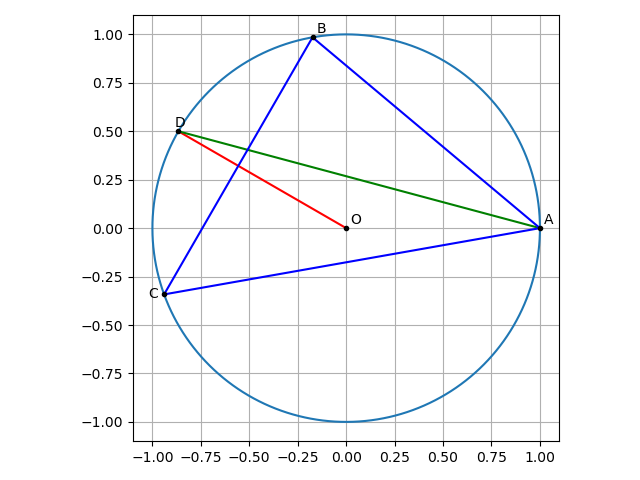
\includegraphics[width=\columnwidth]{figs/angle_perp_bisector.png}
        \caption{The bisector of $\angle A$ and of $BC$ meet on the circumcircle at $D$.}
        \label{fig:perp-angle-bisect}
    \end{figure}
\end{enumerate}
\end{document}
